\documentclass[11pt]{article}
\usepackage[margin=1in]{geometry}
\usepackage{tikz}
\usetikzlibrary{positioning,arrows,fit,backgrounds}

\pgfdeclarelayer{background layer}
\pgfsetlayers{background layer,main}
%===========================================================================================
% #1 ancestor name
% #2 ancestor content
\newcommand{\ancestor}[2]{
	\node [anchor=west] (#1) {#2}
}

% #1 parent name
% #2 index
% #3 child name
% #4 child content
\newcommand{\child}[4]{
	\node [below=#2*5mm of #1.west,anchor=west,xshift=10mm] (#3) {#4};
	\draw [->,thick] (#1.south west) ++(right:3mm)  |- (#3.west)
}

%===========================================================================================
%\setlength{\parindent}{0pt}
\begin{document}

test line testasdf asfasdfsfsdfsdfs asdfsd fakjasdfj asdfkjsakfa adsfjkasfasasdf
asfsf asdfsdf asdfsdfflkfasdf adf kadfjadf asdf asdfjkdasdf fasdf.

\noindent
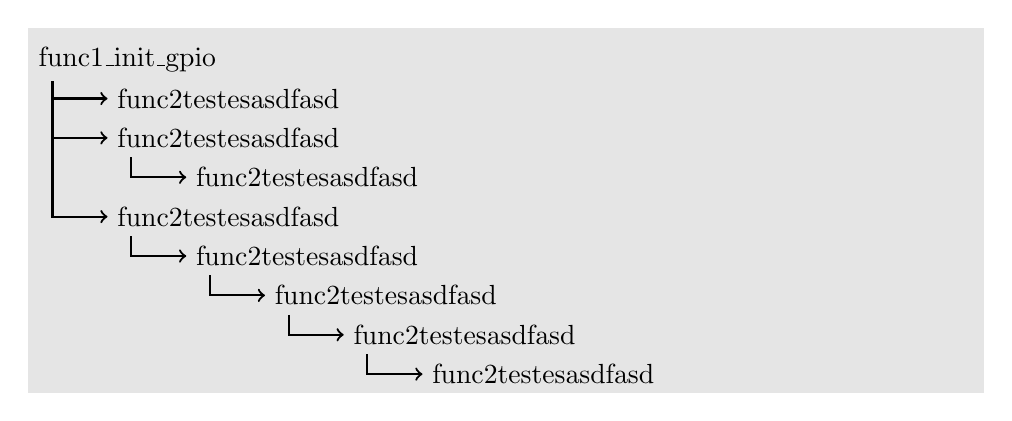
\begin{tikzpicture}
	% On main layer
	\ancestor {f1}{func1\_init\_gpio};
	\child {f1}{1}{f2}{func2testesasdfasd};
	\child {f1}{2}{f3}{func2testesasdfasd};
	\child {f3}{1}{f4}{func2testesasdfasd};
	\child {f1}{4}{f5}{func2testesasdfasd};
	\child {f5}{1}{f6}{func2testesasdfasd};
	\child {f6}{1}{f7}{func2testesasdfasd};
	\child {f7}{1}{f8}{func2testesasdfasd};
	\child {f8}{1}{f9}{func2testesasdfasd};

	% On background layer
	\begin{pgfonlayer}{background layer}
	\fill [gray!20] (current bounding box.south west) rectangle(\textwidth,0.4);
	\end{pgfonlayer}

\end{tikzpicture}

\end{document}
%===========================================================================================
